\chapter{Service-oriented computing}
\label{chap:service-oriented computing}
\emph{Service-oriented computing} represents a distributed computing platform \cite{soa-contract}. It has its own paradigm, logic, architecture and patterns. It is built on the idea of distributed computing platforms and extends it by new considerations about governance, design layers and technologies suitable for its implementation.

\emph{Service orientation} is a design paradigm. It provides separation into logical units which can be utilized according to strategic goals and benefits of a requested target.

\section{Service-oriented architecture}
\emph{Service-oriented architecture (SOA)} is a set of best practices for an organization moving towards \gls{agile} architectural model of the system to meet business needs. Result of applied practices is an architecture which corresponds to dynamic market changes. The SOA best practices describe the human behaviour. There is no list of constraints which have to be followed in order to obtain a service-oriented architecture. The best practices are designed to resolve specific situations which the organization can meet. Just a subset of appropriate practices could be selected.\par

The architecture is layered. There can be multiple layers and they can differ according to the needs of designed system. One of the examples of horizontal layers is shown in figure \ref{fig:soa-architecture}. The layers are separated and each of them encapsulates its implementation so that another layer can't access and modify it (preventing potential harms). In this example is an application containing services which have access to a database using an adapter. The \textit{\gls{adapter}} serves to transform data from a database to data useful for services and vice-versa. \textit{Services} are entry point for consumer's application. They provide access to the data without direct access to \textit{database}.

\begin{figure}[htp] \centering{
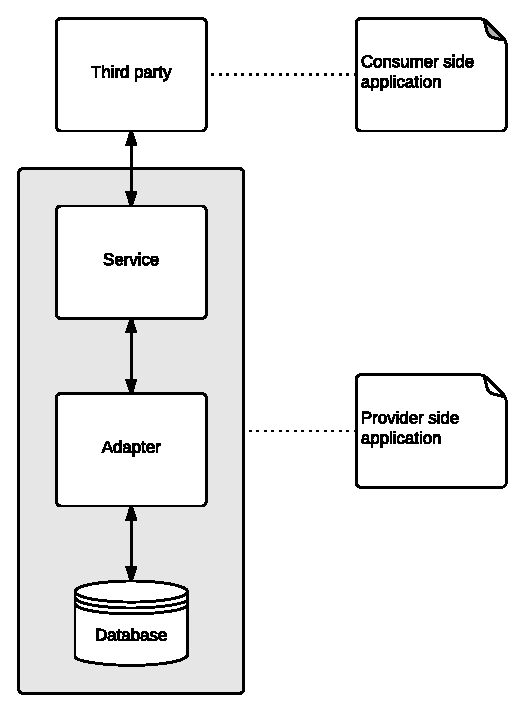
\includegraphics[width=8cm]{img/soa-architecture.pdf}}
\caption{Example of service-oriented architecture model}
\label{fig:soa-architecture}
\end{figure}  

One of the main advantages of a service-oriented architectural style is its ability to efficiently deal with changes. \textit{"SOA is based on a decomposition of enterprise IT assets and separation of 'stable' IT artifacts (services) from 'changeable' artifacts (business processes), orchestrating services into IT solutions (processes)."} \cite{website:versioning-in-soa}.
Above mentioned services are essential part of SOA. Relations between them and a business process constituted by services are visualized in figure \ref{fig:business-process-services}. The business process is a process from the real world and its workflow is simulated by services. A single task of a business process is composed by one or more of the services. Services perform the logic and communicate with underlying layers to retrieve and store data to operate as a business process.

\begin{figure}[htp] \centering{
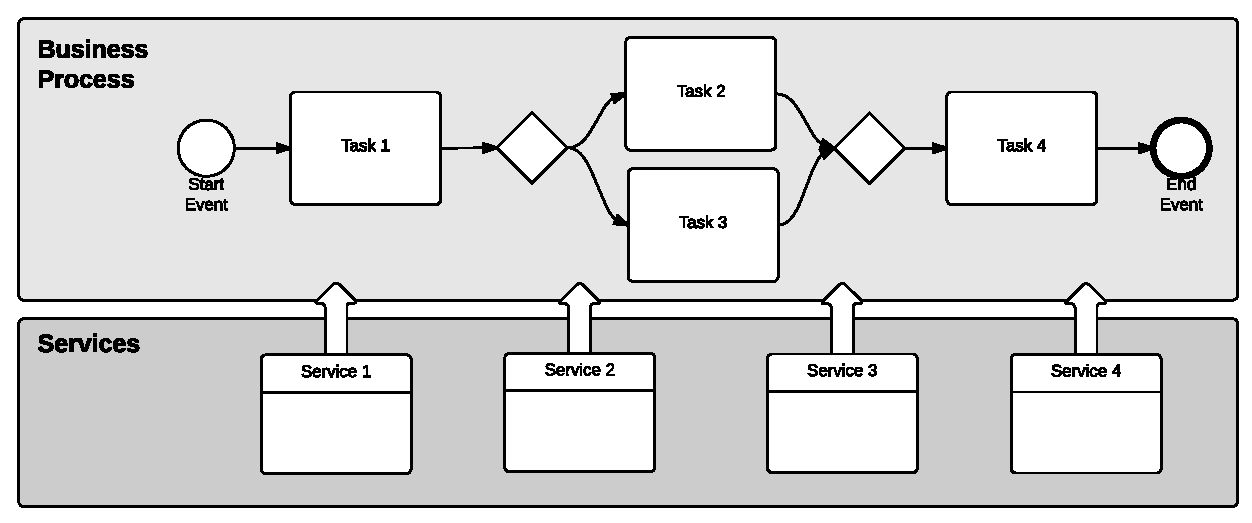
\includegraphics[width=12cm]{img/business-process-services.pdf}}
\caption{Business process as a composition of services}
\label{fig:business-process-services}
\end{figure} 

The speed of changes in the business is too fast to be passed directly into development and maintenance of a \gls{monolithic-systems}. Functionality of these systems is based on measures of a customer and often can't deal with changes easily. It interferes in design of the whole architecture. 

SOA offers better flexibility when business requirements change. Changes are reflected into modifications of an existing business process by changing involved services. If necessary a whole new process is created using existing services. When the existing services do not meet the requirements, a new service can be created. There are more approaches of how to deal with the changes and one of them is versioning described in detail in chapters \ref{chap:versioning} and \ref{chap:versionaccess}.

\section{Services}
\label{sec:services}
SOA is composed from logical units - services. Every service is a standalone object or component. Every service has its own functional context and related capabilities. Each service is deployed independently on other ones and on the system which uses it. It allows a parallel development, one service can be a part of many products of a corporation.
\textit{"The essence of Service in the SOA context is the business abstraction - that is a representation of functionality and/or data presented in business context."} \cite{agile-architecture}

\subsection{Levels of a service} 
\label{subsec:levels-of-service}

It is not completely clear what a service represents. It was already mentioned that it is an abstraction of a business process, but after the analysis stage it is implemented and represented by code.
In fact there are three levels of how the word \emph{Service} can be interpreted in SOA context \cite{agile-architecture}:
\begin{enumerate}
  \item \textbf{Service implementation} \hfill \\
Service implementation is the code containing the logic.
  \item \textbf{Service interface} \hfill \\ 
This level is an entry point to the service implementation, it provides underlying logic to consumers but encapsulates it in a way that consumers can see the implementation. 
  \item \textbf{Abstracted service} \hfill \\
Abstracted service or business service represents a business capability or data. A composition of services describe a business process. This is a core abstraction of SOA.
\end{enumerate}

\begin{figure}[htp] \centering{
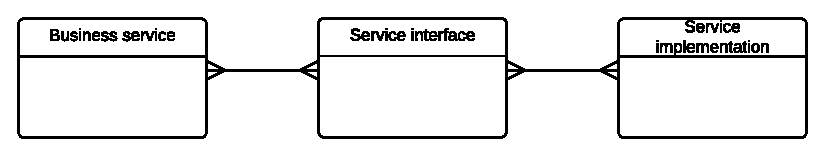
\includegraphics[width=10cm]{img/service-levels.pdf}}
\caption{Relationship between service interpretations}
\label{fig:service-levels}
\end{figure}

There is a many-to-many relationship between these three levels. As can be seen on figure \ref{fig:service-levels} a business service can represent multiple interfaces and in the same time one interface can be supported by multiple implementations.

\subsection{Service lifecycle}
\label{subsec:lifecycle}
The lifecycle of a services passes through several stages. Firstly the business which has to be abstracted by services is analyzed. It defines a set of services and compositions of services abstracting business processes. Than the services can be designed, implemented and tested to work as expected. After that they are deployed and put into use of a consumer. Deployed and consumed services are maintained and monitored by their provider. Monitoring helps to improve the services. Finally services are versioned. A new version of a service can be implemented and the old one is retired.

Diagram with the stages is shown in figure \ref{fig:service-lifecycle}. Here are the stages of service lifecycle as they are defined by Thomas Erl \cite{soa-governance}:

\begin{figure}[htp] \centering{
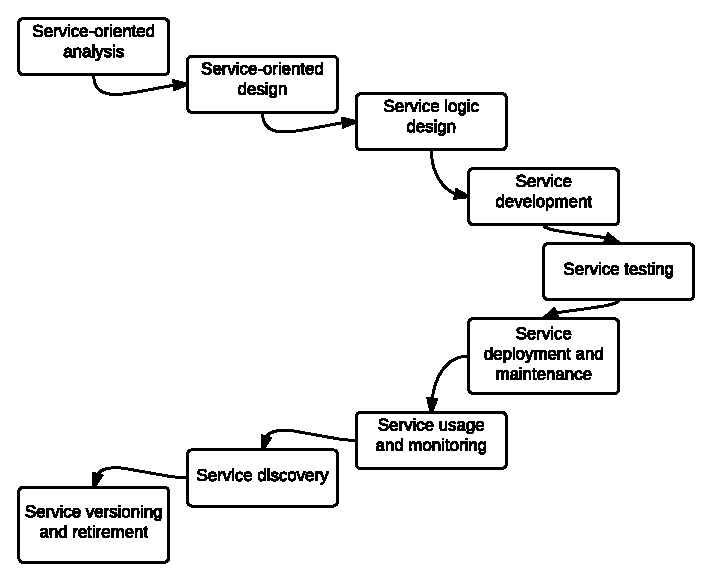
\includegraphics[width=10cm]{img/service-lifecycle.pdf}}
\caption{Service lifecycle stages}
\label{fig:service-lifecycle}
\end{figure}


\begin{enumerate}
  \item Service-oriented analysis \\
  During this phase the services candidates, their capabilities and compositions are created. The analysis is typically iterative, for each business process one service inventory is created.
  \item Service-oriented design \\
  This stage designs the service contracts. For every service candidate it is considered a technical contract, in case of REST services (described in chapter \ref{chap:rest}). It is inevitable to think of HTTP methods usage, resource identifiers and header parameters.
  \item Service Logic Design \\
  Service architecture and its logic is established, so that the service will carry out the functionality which results from the contract.
  \item Service Development \\
  Implementation of the services is performed. It is based on the specifications and architecture design from previous stages.
  \item Service Testing \\
  The implemented services need to be tested in order to provide the quality assurance of developed application.
  \item Service Deployment and Maintenance \\
  In this phase the services are deployed on a production environment. Maintenance involves changes and upgrades of services related to production environment, but it doesn't include changes which would result in a new version of services.
  \item Service Usage and Monitoring \\
  Deployed service which is in use is an object of monitoring. It is essential for obtaining various metrics. Measured values can positively influence the maintenance and are further used for business assessments.
  \item Service Discovery \\
  Process of identifying \gls{agnostic-services} throughout the given service inventory.
  \item Service Versioning and Retirement \\
  After deployment and usage a need to change the logic or addition of a new service can arise. How to version the services will be explained in chapter \ref{chap:versioning}. 
  
  Retirement encompasses the termination of a service usage. Regarding service versioning a version of service which is no longer in use can be retired.
\end{enumerate}


\bigskip

\subsection{Service granularity}
\label{sec:granularity}
In SOA context granularity is an often used expression. Granularity of an entity represents amount of data which is understood as one unit related to the whole data pool. It is possible to distinguish from fine-grained to coarse-grained granularity. Where fine-grained contains small amount of data in one unit respective to whole data pool. On the contrary the coarser granularity bears much more data in one unit.

Service granularity is defined during analytical part of the service design. Granularity determines properties of the services related to the business process. Services can be fine-grained up to coarse-grained. When services are fine-grained number of services is higher and they contain less logic. Therefore the cost of the implementation is smaller and the higher reusability is provided. However the effort needed to compose these services into a process is higher. 

On the other side when services are coarse-grained they contain more complex logic and easily compose the process. However reusability is limited and more effort is required to implement them.

The example of fine-grained and coarse-grained granularity can be shown on a simple business process. An update user process is visualized on the figure \ref{fig:granularity}.

\begin{figure}[htp] \centering{
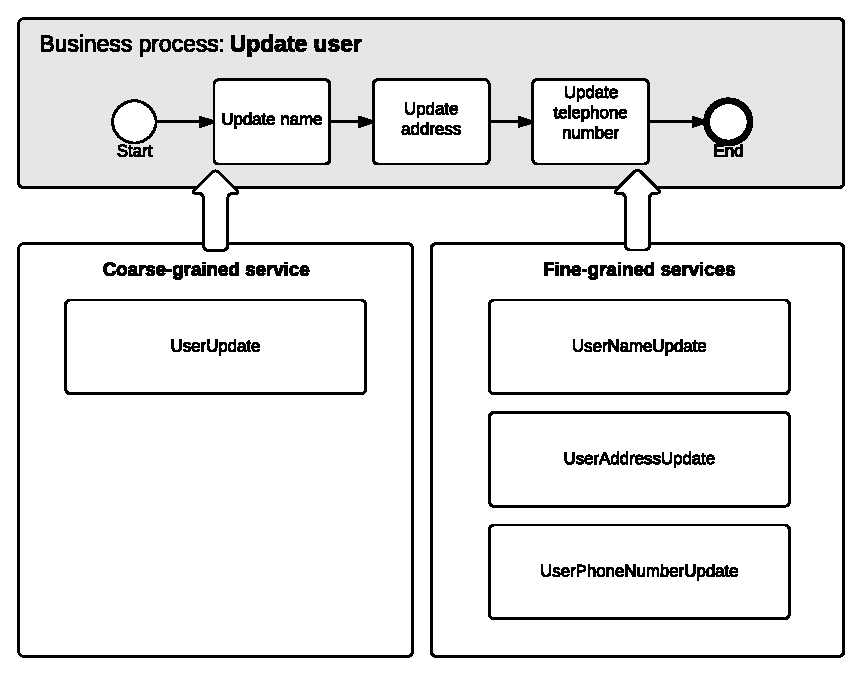
\includegraphics[width=12cm]{img/granularity.pdf}}
\caption{Coarse-grained and fine-grained services}
\label{fig:granularity}
\end{figure}

The coarse-grained service contains more logic. One service is responsible for whole process. The service executes update of user's name, address and phone number by itself. Advantage is less interaction between client and server. However the service is less flexible because of fixed steps. If there is a need to add a one more step into the process the service will have to be changed.

On the other side the process could be composed of fine-grained services. One service is responsible for less logic. Update process is than a composition of services UpdateName, UpdateAddress, UpdatePhoneNumber. In this case there is more interaction between client and server - there are three services called one by one. On the other hand services are flexibly composed and can be rearranged. If there is a need to add an additional step in the process a new service will be added.


\subsection{Web services}
Web services are one group of services, these are intended to work on a network. They are components of \gls{web-applications}. Web services can be designed using different styles. The most popular nowadays is Representational State Transfer (REST) architectural style. This thesis deals with REST architectural style and REST services. They will be described in detail within chapter \ref{chap:rest}.


